\section{eo\-SGA$<$ EOT $>$ Class Template Reference}
\label{classeo_s_g_a}\index{eoSGA@{eoSGA}}
The Simple Genetic Algorithm, following Holland and Goldberg.  


{\tt \#include $<$eo\-SGA.h$>$}

Inheritance diagram for eo\-SGA$<$ EOT $>$::\begin{figure}[H]
\begin{center}
\leavevmode
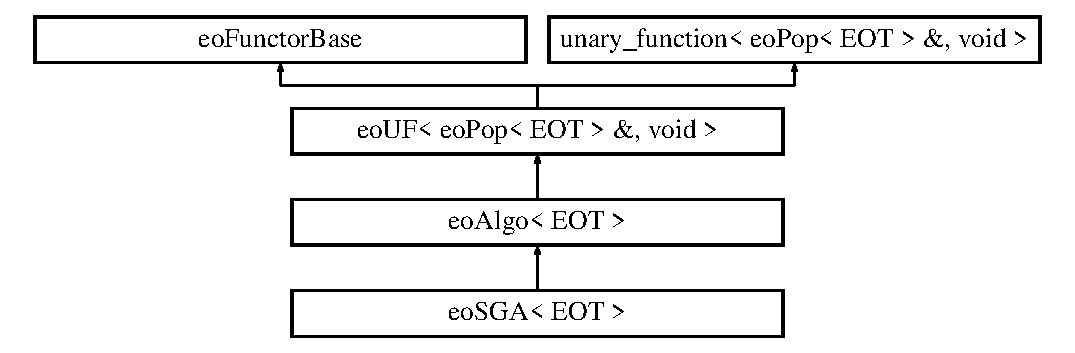
\includegraphics[height=4cm]{classeo_s_g_a}
\end{center}
\end{figure}
\subsection*{Public Member Functions}
\begin{CompactItemize}
\item 
{\bf eo\-SGA} ({\bf eo\-Select\-One}$<$ {\bf EOT} $>$ \&\_\-select, {\bf eo\-Quad\-Op}$<$ {\bf EOT} $>$ \&\_\-cross, float \_\-crate, {\bf eo\-Mon\-Op}$<$ {\bf EOT} $>$ \&\_\-mutate, float \_\-mrate, {\bf eo\-Eval\-Func}$<$ {\bf EOT} $>$ \&\_\-eval, {\bf eo\-Continue}$<$ {\bf EOT} $>$ \&\_\-cont)\label{classeo_s_g_a_a0}

\item 
void {\bf operator()} ({\bf eo\-Pop}$<$ {\bf EOT} $>$ \&\_\-pop)\label{classeo_s_g_a_a1}

\begin{CompactList}\small\item\em The pure virtual function that needs to be implemented by the subclass. \item\end{CompactList}\end{CompactItemize}
\subsection*{Private Attributes}
\begin{CompactItemize}
\item 
{\bf eo\-Continue}$<$ {\bf EOT} $>$ \& {\bf cont}\label{classeo_s_g_a_r0}

\item 
{\bf eo\-Invalidate\-Mon\-Op}$<$ {\bf EOT} $>$ {\bf mutate}\label{classeo_s_g_a_r1}

\begin{CompactList}\small\item\em {\bf eo\-Invalidate\-Mon\-Op}{\rm (p.\,\pageref{classeo_invalidate_mon_op})} invalidates the embedded operator \item\end{CompactList}\item 
float {\bf mutation\-Rate}\label{classeo_s_g_a_r2}

\item 
{\bf eo\-Invalidate\-Quad\-Op}$<$ {\bf EOT} $>$ {\bf cross}\label{classeo_s_g_a_r3}

\item 
float {\bf crossover\-Rate}\label{classeo_s_g_a_r4}

\item 
{\bf eo\-Select\-Perc}$<$ {\bf EOT} $>$ {\bf select}\label{classeo_s_g_a_r5}

\item 
{\bf eo\-Eval\-Func}$<$ {\bf EOT} $>$ \& {\bf eval}\label{classeo_s_g_a_r6}

\end{CompactItemize}


\subsection{Detailed Description}
\subsubsection*{template$<$class EOT$>$ class eo\-SGA$<$ EOT $>$}

The Simple Genetic Algorithm, following Holland and Goldberg. 

Needs a selector (class {\bf eo\-Select\-One}{\rm (p.\,\pageref{classeo_select_one})}) a crossover (eo\-Quad, i.e. a 2-$>$2 operator) and a mutation with their respective rates, of course an evaluation function ({\bf eo\-Eval\-Func}{\rm (p.\,\pageref{classeo_eval_func})}) and a continuator ({\bf eo\-Continue}{\rm (p.\,\pageref{classeo_continue})}) which gives the stopping criterion. Performs full generational replacement. 



Definition at line 49 of file eo\-SGA.h.

The documentation for this class was generated from the following file:\begin{CompactItemize}
\item 
eo\-SGA.h\end{CompactItemize}
